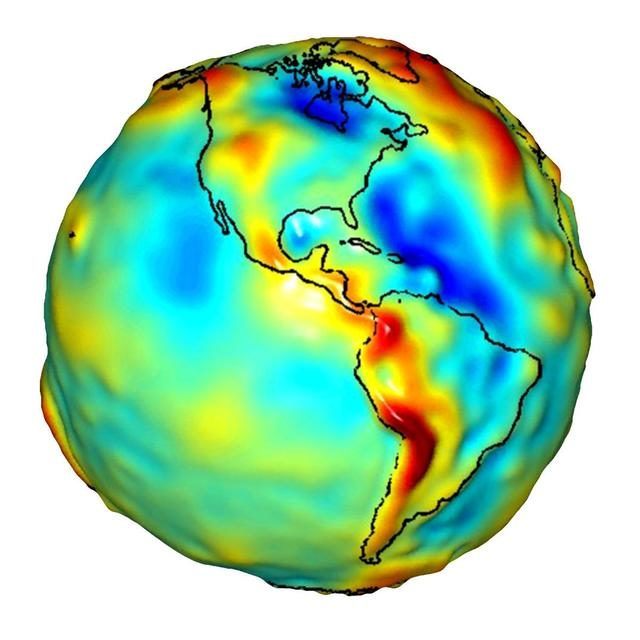
\includegraphics[height=1.25cm]{images/pictograms/gravity}

\includegraphics[height=1.25cm]{images/pictograms/benchmark}

%%%%%%%%%%%%%%%%%%%%%%%%%%%%%%%%%%%%%%%%%%%%%%%%%%%%%%%%%%%%%%%%%%%%%%%%%%%%%%%%%%%%%%%%%%%%%%%%%%%

\begin{flushright} {\tiny {\color{gray} python\_codes/fieldstone\_132/text.tex}} \end{flushright}

\lstinputlisting[language=bash,basicstyle=\small]{python_codes/fieldstone_132/keywords.ascii}

\begin{center}
\inpython
Code: \url{https://github.com/cedrict/fieldstone/tree/master/python_codes/fieldstone_132}
\end{center}

\par\noindent\rule{\textwidth}{0.4pt}
%%%%%%%%%%%%%%%%%%%%%%%%%%%%%%%%%%%%%%%%%%%%%%%%%%%%%%%%%%%%%%%%%%%%%%%%%%%%%%%%%%%%%%%%%%%%%%

Let us consider a circle of mass M in the $(x,y)$-plane of radius $R$ centered at the origin.
Let us consider a point $P$ of coordinates $(x_P,y_P,z_P)$ at which we compute the 
gravity field generated by the circle:

\begin{center}
\includegraphics[width=7cm]{python_codes/fieldstone_132/images/setup.png}\\
{\captionfont Redo FIGURE}
\end{center}

We are considering a small element of the ring of mass $\delta m$ (with $\oint dm = M$). 
The contribution of this element to the field is
\[
\delta \vec{g} = \frac{{\cal G} \delta m}{d^2} \vec{e}_{MP}
\]

In what follow we arbitrarily set the linear density to $\rho=10^6~\si{\kg\per\meter}$ and 
the radius of the circle to $R=1.123$

%----------------------------------------------------------------
\subsection*{Case 1: $P$ is above the center of the circle}

In this case:
\[
d=\sqrt{R^2 + z_P^2}
\]
and because of symmetry we know that the resulting 
gravity components $g_x$ and $g_y$ will be zero.

\begin{center}
\includegraphics[width=9cm]{python_codes/fieldstone_132/results/case1/setup.pdf}
\end{center}

For the mass $\delta m$ the contribution on the $z$-axis is given by 
\[
\delta g_z = \frac{{\cal G} \delta m}{R^2+z_P^2} \cos\theta 
\] 
We see that 
\[
\cos\theta = \frac{z_P}{\sqrt{R^2+z_P^2}}
\]
so that
\[
\delta g_z = \frac{{\cal G} \delta m}{R^2+z_P^2}\frac{z_P}{\sqrt{R^2+z_P^2}}
\] 
By integrating this expression for the entire circle we 
find\footnote{See also video \url{https://www.youtube.com/watch?v=q5EWLNdv_pE}}:
\[
g_z=\frac{{\cal G} M z_P}{(R^2+z_P^2)^{3/2}}
\]

\begin{center}
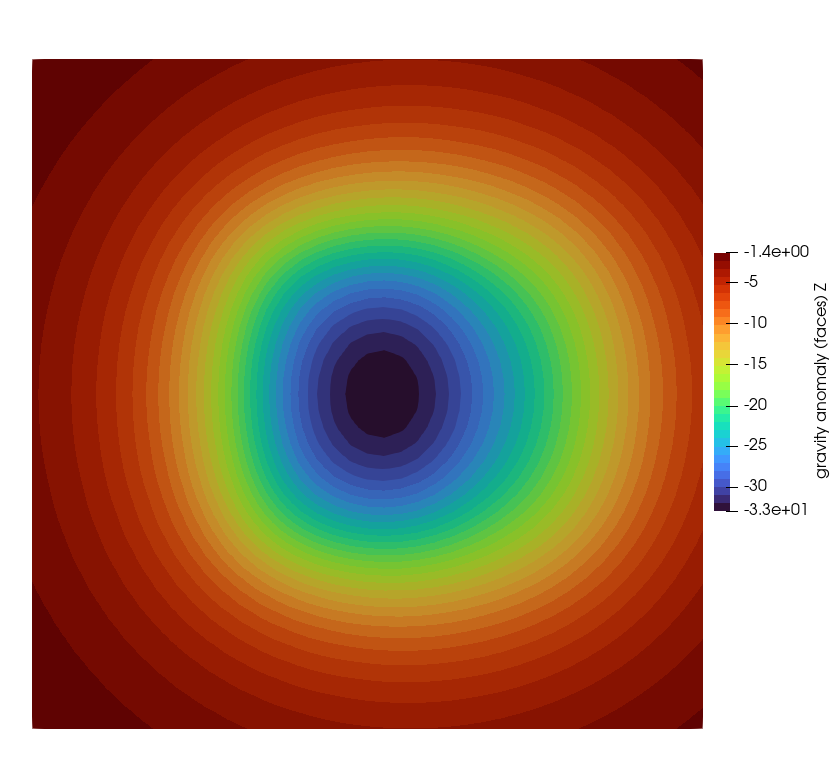
\includegraphics[width=9cm]{python_codes/fieldstone_132/results/case1/gz.pdf}\\
{\captionfont Vertical component of the gravity field as a function of $z$, 
for various circle resolution, plotted against the analytical solution.}
\end{center}



%----------------------------------------------------------------
\subsection*{Case 2: $P$ is in the plane circle}

Unfortunately I was not able to find or derive an analytical solution for this case.
Gravity is measured on a line starting at the center of the circle, following the 
$x$-axis and up to $x=2R$:

\begin{center}
\includegraphics[width=7cm]{python_codes/fieldstone_132/results/case2/setup.pdf}
\end{center}

\begin{center}
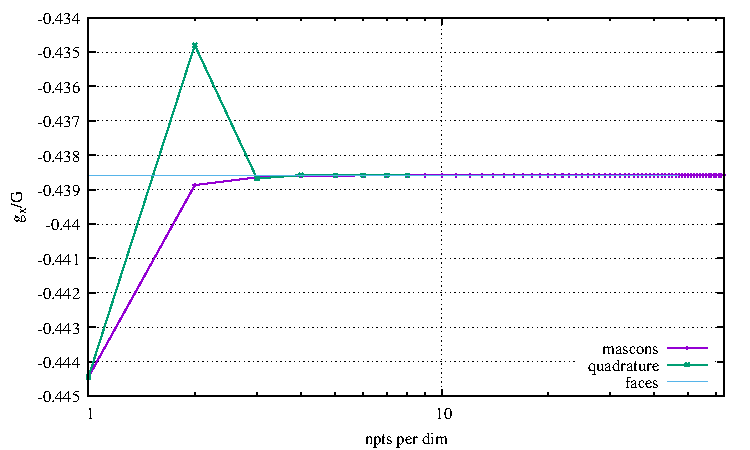
\includegraphics[width=5.7cm]{python_codes/fieldstone_132/results/gx.pdf}
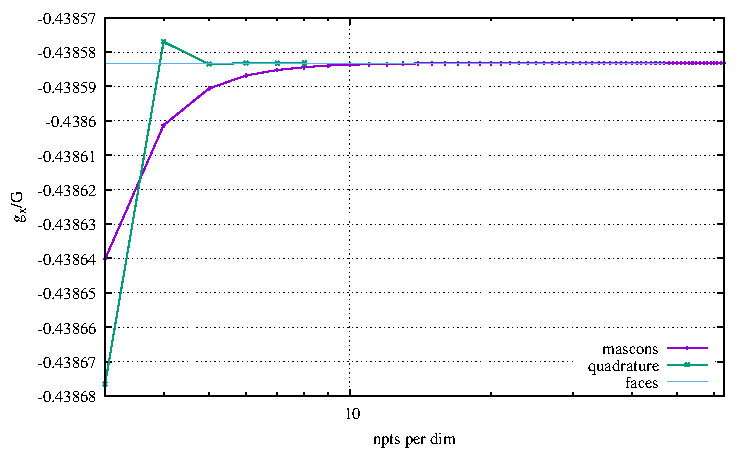
\includegraphics[width=5.7cm]{python_codes/fieldstone_132/results/gx2.pdf}
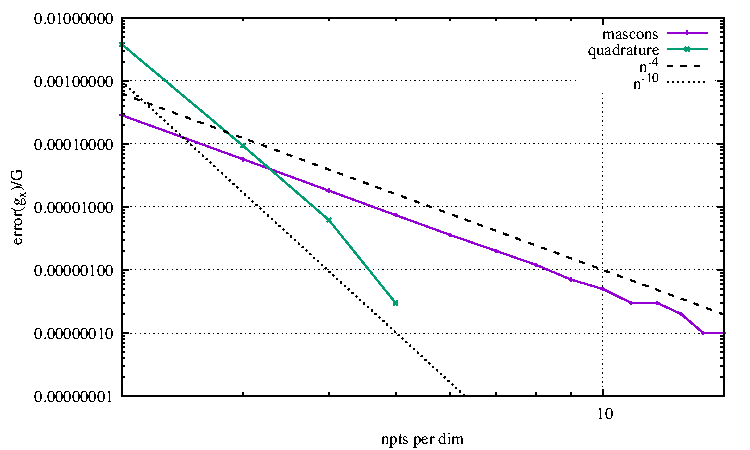
\includegraphics[width=5.7cm]{python_codes/fieldstone_132/results/gx3.pdf}
\end{center}
